\iffalse
https://edoc.sub.uni-hamburg.de/hcu/volltexte/2017/370/pdf/Ebert_Kirsten.pdf Anfang
\fi

Im folgendem werde ich Verkäufer aller Art ähnlich wie im Buch "Das E-Commerce Buch: Marktanalysen - Geschäftsmodelle - Strategien" unterteilen: in Online-Marktplätze, Online-Händler, Kataloversender, stationäre Händler und Hersteller\cite[S. 15ff]{Graf}. Dabei sind Online-Marktplätze eine Art Online-Vermittler zwischen Kunden und Verkäufer, Online-Händler bieten dagegen nur eigene, meist sehr spezialisierten Sortimente an. Kataloversender verhalten sich ähnlich: sie versenden ihr Sortiment direkt an Kunden. Stationäre Händler verkaufen im Gegensatz zu den genannten Vertreibsstrukturen in Fillialen und sind mit Kataloghändlern am stärksten von den Änderungen der letzten Jahrzenten betroffen. Während sich die genannten Unternehmensarten meistens am Ende der Verkaufskette befinden, stehen Händler oft am Anfang: sie stellen Güter her und sind dementsprechend, insofern sie nicht selber verkaufen, auf weitere Unternehmen für Verkauf und Vermarktung angewiesen(ebd.). %vor und -nachteile?; beispielsunternehmen

% KATALOGHÄNDLER

Kataloghändler sind die größten Verlierer der letzten Jahrzehnte: mit der Entwicklung des Onlinehandels ist ab 2002 schon ein Rückgang der Nachfrage zu spüren – einige eröffnen eigene Online-Shops\cite[S. 24f]{Graf}, jedoch oft mit wenig Erfolg\cite[S. 38]{Graf}. 2015 sind Katalogversender fast ausschließlich verschwunden oder zu Online- und Einzelhandel konvertiert, da sie kaum einen Mehrwert im Vergleich zum klassisschen Onlinehandel bieten\cite[S. 47]{Graf}.

% STATIONÄR
    % nitt S 54 these, dass einzelhandel zurückkommt
Der stationäre Handel ist durch die steigende Relevanz des Onlinehandels auch weniger gefragt denn je und versucht mit strukturellen Änderungen dagegen anzukämpfen. Einige Einzelhändler eröffenen paralel zu ihrem Geschäft einen Online-Shop, andere bieten die Möglichkeit, Waren online in den Laden zu bestellen und diese dort anzuholen – sogenanntes "Multichannel-Marketing", das Ansprechen der Kunden über mehrere Wege\cite[S. 34f]{Graf}. Jedoch fahren die neuen Strkturen nur wenig Erfolge ein – so erhöhen sie zwar die Onlinepräsenz, bieten jedoch nur einen geringen Mehrwert im Vergleich zu den bekannten Onlineriesen wie Amazon\cite[S. 34f]{Graf}. 
Allerdings hat der stationäre Handel in der Theorie noch einen bedeutenden Vorteil: den sozialen Aspekt. Dieser wird vermutlich mit fortschreitender Digitalisierung eine immer wichtigere Rolle spielen\cite[S. 50]{Ebert}.
\begin{quote}
"Als Mittel gegen Vereinsamung und Anonymisierung im Alltag wird die soziale Komponente beim Einkaufen [...] zunehmend an Bedeutung gewinnen."\cite[S. 43]{Nitt}
\end{quote} 
Außerdem gibt es beim Einzelhandel Bereiche, die nicht oder nur schwer durch andere Vertriebswege abzudecken sind, wie 

% ONLINE

Die Onlinehändler und -marktplätze sind die Gewinner der letzten 20 Jahre – die Verkäufswerte wuchsen ab der Jahrtausendwende konstant an und stellen in vielen Branchen für andere Vertriebsstrukturen eine ernst zu nehmende Konkurrenz dar\cite{wolf}. Vorerst wechseln Konsumenten von Katalogen, ab 2010 auch viele Nutzer anderer Verkaufswege, da das Kaufen online fast immer einen Preisvorteil bietet\cite[S. 31]{Graf}.
\begin{figure}[h]
    \begin{center}
        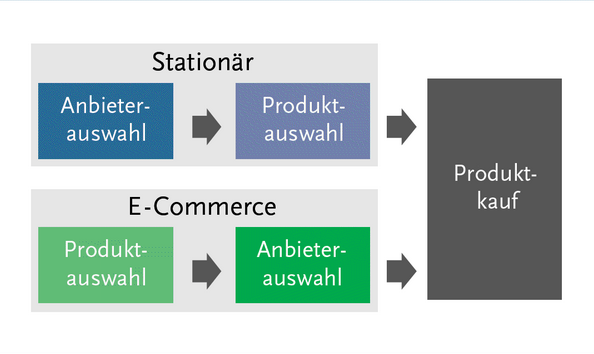
\includegraphics[width=8cm]{media/Fabian-konsumwandel.png}
        \caption{Kaufprozess im Vergleich – Stationär und E-Commerce}
        \label{konsumwandel}
        \bildquelle Björn Schäfers, Social Shopping für Mode, Wohnen und Lifestyle am Beipiel Smatch.com in Web-Exzellenz im E-Commerce, Gabler, S. 313 %lieber quelle e com buch???
    \end{center}
\end{figure} 
Außerdem hat sich unter Nutzern des Onlinehandels ein neues Konsumverhalten entwickelt. Bis dahin wa es üblich, zuerst den Anbieter, danach das zu kaufende Produkt auszuwählen; jedoch hat der Onlinehandel dieses Verhalten invertiert, da das Vergleichen mehrerer Anbieter im Internet um ein vielfaches einfacher ist als stationär\cite[S 22f]{Graf}. 
Neu unter Konsumenten ist auch das Bedürfnis nach individiuellen und auf den Käufer angepassten Produkten\cite[S. 43]{Nitt}, was wahrscheinlich durch die extrem große Außwahl bei dem Online-Shopping ausgelöst wurde. In diesem Aspekt kann der stationäre Einzelhandel schlicht nicht mithalten, da Raum für Produkte begrenzt und preisintensiv ist. 

% HERSTELLER

Ähnlich wie der Einzelhandel sehen Hersteller den Onlinehandel zuerst in einem negativen Licht - aufgrund von untransparenten Verkäufern und möglichen negativen Imageeffekten\cite[S. 20]{Graf}. Außerdem entstehen 2002 erste, sogenannte "Powerseller", die im Großhandel Markenprodukte kaufen und deutlich unterhalb des Einzelhandels-Preisniveaus verkaufen\cite[S. 26]{Graf}. Mit der Zeit bauen Marken verzögert, aber schneller als der Einzelhandel immer mehr eigene Verkaufsportale, um ihre Güter direkt ohne eine Zwischeninstanz zu verkaufen und steigern ihren Umsatz damit bedeutend – beispielsweise verlässt Hugo Boss 2013 Zalando um Produkte über die Website hugoboss.com zu verkaufen\cite[S. 48f]{Graf}. Außerdem wird durch das direkte Feedback eine bessere Produktentwicklung und Kundensupport ermöglicht\cite[S. 39]{Graf}. 

% ALLGEMEIN

Das Konsumverhalten hat sich auch unabhängig von der Vertriebsstruktur geändert: statt gleichbleibenden, rationalen Käufen und Kaufmotiven, die die Auswahl der gekauften Güter stark abhängig von der zur Verfügung stehenden Geldmenge machten\cite[S. 38]{Schramm}; herrscht heute ein deutlich dynamischeres Kaufklima:
\begin{quote}
"So beziehen jetzt zum Beispiel auch solvente Kunden ihre Lebensmittel aus dem Billigdiscounter, während  umgekehrt  einkommensschwächere  Schichten  zu  Luxusgütern  greifen."\cite[S. 43]{Nitt}
\end{quote}
Außerdem gibt es kaum noch "pure" Einzelhändler und Onlinehändler – meist sind Firmen in mehreren Bereichen vertreten, um ihre Präsenz zu steigern. So eröffnet etwa Amazon in den letzen Jahren Läden vor Ort und stationäre Händler betreiben Online-Shops\cite[S. 50]{Graf}.
Außerdem ist das Konsumverhalten in Deutschlands seit Jahren durch eine starke Kaufkraft geprägt, z. T. dank dem 0\%-igen Leitzins der \ac{EZB}\cite[S. 49]{Ebert} – auch wenn die derzeitige Corona-Situation diese leicht abgeschwächt hat\cite{BfWE}. 

\iffalse 
       
        auch ältere kaufen online ein: evilcom S 8
        
    
        
        allgemein online: großes wachstum ab 2002 S. 26
            jüngere kaufen mehr online ein S 35f
            kleinere haben wenig chancen, da große wie amazon durch hohes kapital niedrige preise finanzieren können, was einer der wichtigsten faktoren beim onlinehandel ist S 37f
            dropshipping: verkauf über händler, versand direkt von hersteller: lagerkosten: n.a.
            datenbeschaffung: bessere produktempfehlungen, infos über kaufverhalten und mögl. dynamische preise
            
    
        
        Stationär----------------------------------------------------------------


            einzelhandel weniger preissensibel; jedoch ist onlinehandel vor allem in der Elektronikbranche konkurrenzfähig, sh. Media Markt\cite[S. 21f]{Graf}

        gute bereiche: essen und beratungsintensives
        gründe, stationär zu kaufen: beratung, feeling
            deutliche verluste ab 2019 S 31
            
            erste onlnie-shops S 30
            
            lebensmittel fast ausschließlich stationär: aber "Picnic" fährt mit robotern die innenstädte ab: S 51


            
\fi








\iffalse
> billig - strategie vorallem von amazon und alibaba

veranschaulichung eigene tabelle börsenwert einzelner unternehmen

Dabei gibt es auch unternehmen, die mehrere berieche nutzen, wie amazon
\fi





%ergebnisse: kataloghandel kann kaum noch bestehen



\iffalse WIRTSCHAFT
allgemein:
        push ist obsolet > pull S 51
        
 Hersteller: sogenannte "Powerseller" kaufen produkte direkt von herstellern, verkaufen sie deutlich unter marktpreisen weiter -> probleme mit preisverfall S. 25
        schrecken aufgrund von biosherigen vertreib über fachhandel meist davor zurück, online-marktplätze einzurichten, vereinzelt(hugoboss.com) S. 30
            "wechseln von b2b zu b2c, sprich bieten waren direkt an, preisvorteil" für billigere preise
        stärker ab 2012, aber powerseller problem S 39f
zuerst ist onlinehandel herausforderung, da "Preis und Leistung der Online-Verkäufer sind praktisch nicht kontrollierbar und undurchsichtig für Marken und Hersteller. Außerdem fürchten die Hersteller einen Kontrollverlust des Markenauftrittes und negative Imageeffekte." S 20



       online----------------------------------------------------------
            hohe retourkosten, neueinsteiger haben es schwierig S 46f
\fi
